    \documentclass[../main.tex]{subfiles}

\begin{document}

\chapter{Roundoff and Truncation Errors}
\label{chap:chap_4}

\begin{center}
\Large{\textbf{CHAPTER OBJECTIVES}}    
\end{center}
The primary objective of this chapter is to acquaint you with the major sources of
errors involved in numerical methods. Specific objectives and topics covered are
\begin{itemize}
\item Understanding the distinction between accuracy and precision.
\item Learning how to quantify error.
\item Learning how error estimates can be used to decide when to terminate an iterative
calculation.
\item Understanding how roundoff errors occur because digital computers have a
limited ability to represent numbers.
\item Understanding why floating-point numbers have limits on their range and
precision.
\item Recognizing that truncation errors occur when exact mathematical formulations
are represented by approximations.
\item Knowing how to use the Taylor series to estimate truncation errors.
\item Understanding how to write forward, backward, and centered finite-difference
approximations of first and second derivatives.
\item Recognizing that efforts to minimize truncation errors can sometimes increase
roundoff errors.
\end{itemize}

\bigskip
\noindent
\Large{YOU'VE GOT A PROBLEM}
\bigskip

\noindent
\normalsize{In Chap. 1 you developed a numerical model for the velocity of a bungee jumper. To
solve the problem with a computer, you had to approximate the derivative of velocity
with a finite difference.}

\bigskip
$\dfrac{dv}{dt}\cong\dfrac{\mid\Delta v}{\Delta t}=
\dfrac{v(t_{i+1})-v(t_i)}{t_{i+1}-t_i}$

\bigskip
\noindent
Thus, the resulting solution is not exact --- that is, it has error.

In addition, the computer you use to obtain the solution is also an imperfect tool. Because
it is a digital device, the computer is limited in its ability to represent the magnitudes
and precision of numbers. Consequently, the machine itself yields results that contain error.

So both your mathematical approximation and your digital computer cause your resulting
model prediction to be uncertain. Your problem is: How do you deal with such uncertainty?
In particular, is it possible to understand, quantify and control such errors in
order to obtain acceptable results? This chapter introduces you to some approaches and
concepts that engineers and scientists use to deal with this dilemma.

\bigskip
\section[ERRORS]{ERRORS}

\noindent Engineers and scientists constantly find themselves having to accomplish objectives based
on uncertain information. Although perfection is a laudable goal, it is rarely if ever attained.
For example, despite the fact that the model developed from Newton's second law
is an excellent approximation, it would never in practice exactly predict the jumper's fall.
A variety of factors such as winds and slight variations in air resistance would result in deviations
from the prediction. If these deviations are systematically high or low, then we
might need to develop a new model. However, if they are randomly distributed and tightly
grouped around the prediction, then the deviations might be considered negligible and the
model deemed adequate. Numerical approximations also introduce similar discrepancies
into the analysis.

This chapter covers basic topics related to the identification, quantification, and minimization
of these errors. General information concerned with the quantification of error is
reviewed in this section. This is followed by Sections 4.2 and 4.3, dealing with the two
major forms of numerical error: roundoff error (due to computer approximations) and truncation
error (due to mathematical approximations). We also describe how strategies to reduce
truncation error sometimes increase roundoff. Finally, we briefly discuss errors not
directly connected with the numerical methods themselves. These include blunders, model
errors, and data uncertainty.

\subsection{Accuracy and Precision}
\noindent
The errors associated with both calculations and measurements can be characterized with
regard to their accuracy and precision. Accuracy refers to how closely a computed or measured
value agrees with the true value. Precision refers to how closely individual computed
or measured values agree with each other.

These concepts can be illustrated graphically using an analogy from target practice.
The bullet holes on each target in Fig. 4.1 can be thought of as the predictions of a numerical
technique, whereas the bull's-eye represents the truth. Inaccuracy (also called bias) is
defined as systematic deviation from the truth. Thus, although the shots in Fig. 4.1c are
more tightly grouped than in Fig. 4.1a, the two cases are equally biased because they are
both centered on the upper left quadrant of the target. Imprecision (also called uncertainty),
on the other hand, refers to the magnitude of the scatter. Therefore, although Fig. 4.1b and
d are equally accurate (i.e., centered on the bull's-eye), the latter is more precise because
the shots are tightly grouped.

\begin{figure}[h]
    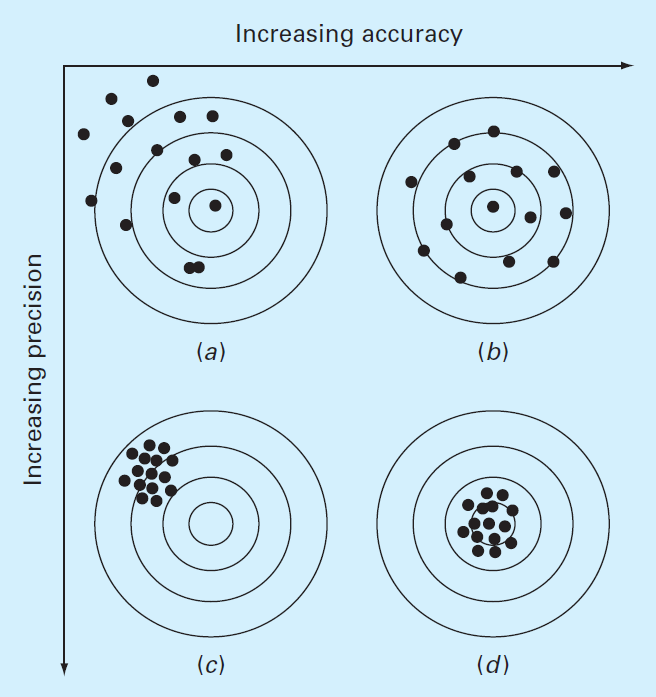
\includegraphics[width=0.55\linewidth]{./images/fig_4_1.png}    
    \caption{An example from marksmanship illustrating the concepts of accuracy and precision:
    (\emph{a}) inaccurate and imprecise, (\emph{b}) accurate and imprecise, (\emph{c}) inaccurate and precise,
    and (\emph{d}) accurate and precise.}
\end{figure}

\bigskip
Numerical methods should be sufficiently accurate or unbiased to meet the requirements
of a particular problem. They also should be precise enough for adequate design.
In this book, we will use the collective term \emph{error} to represent both the inaccuracy and
imprecision of our predictions.

\subsection{Error Definitions}
\noindent
Numerical errors arise from the use of approximations to represent exact mathematical operations
and quantities. For such errors, the relationship between the exact, or true, result
and the approximation can be formulated as
\newline

True value = approximation + error
\hfill
(4.1)
\newline

\noindent
By rearranging Eq. (4.1), we find that the numerical error is equal to the discrepancy
between the truth and the approximation, as in
\newline

$E_t$ = true value - approximation
\hfill
(4.2)
\newline

\noindent
where $E_t$ is used to designate the exact value of the error. The subscript t is included to designate
that this is the ``true'' error. This is in contrast to other cases, as described shortly,
where an ``approximate'' estimate of the error must be employed. Note that the true error is
commonly expressed as an absolute value and referred to as the \emph{absolute error}.

A shortcoming of this definition is that it takes no account of the order of magnitude of
the value under examination. For example, an error of a centimeter is much more significant if we are measuring a rivet than a bridge. One way to account for the magnitudes of the
quantities being evaluated is to normalize the error to the true value, as in$\mid$
\newline

True fractional relative error = $\dfrac{\text{true value -- approximation}}{\text{true value}}$
\newline

\noindent
The relative error can also be multiplied by 100\% to express it as
\newline

$\epsilon_t = \dfrac{\text{true value -- approximation}}{\text{true value}} 100\%$
\hfill
(4.3)
\newline

\noindent
where $\epsilon_t$ designates the true percent relative error.

For example, suppose that you have the task of measuring the lengths of a bridge and
a rivet and come up with 9999 and 9 cm, respectively. If the true values are 10,000 and
10 cm, respectively, the error in both cases is 1 cm. However, their percent relative errors
can be computed using Eq. (4.3) as 0.01\% and 10\%, respectively. Thus, although both measurements
have an absolute error of 1 cm, the relative error for the rivet is much greater. We
would probably conclude that we have done an adequate job of measuring the bridge,
whereas our estimate for the rivet leaves something to be desired.

Notice that for Eqs. (4.2) and (4.3), $E$ and $\epsilon$ are subscripted with a \emph{t} to signify that the
error is based on the true value. For the example of the rivet and the bridge, we were provided
with this value. However, in actual situations such information is rarely available.
For numerical methods, the true value will only be known when we deal with functions that
can be solved analytically. Such will typically be the case when we investigate the theoretical
behavior of a particular technique for simple systems. However, in real-world applications,
we will obviously not know the true answer \emph{a priori}. For these situations, an
alternative is to normalize the error using the best available estimate of the true value --- that
is, to the approximation itself, as in
\newline

$\epsilon_a = \dfrac{\text{approximate error}}{\text{approximation}}100\%$
\hfill
(4.4)
\newline

\noindent
where the subscript a signifies that the error is normalized to an approximate value. Note
also that for real-world applications, Eq. (4.2) cannot be used to calculate the error term in
the numerator of Eq. (4.4). One of the challenges of numerical methods is to determine
error estimates in the absence of knowledge regarding the true value. For example, certain
numerical methods use \emph{iteration} to compute answers. In such cases, a present approximation
is made on the basis of a previous approximation. This process is performed repeatedly,
or iteratively, to successively compute (hopefully) better and better approximations.
For such cases, the error is often estimated as the difference between the previous and present
approximations. Thus, percent relative error is determined according to
\newline

$\epsilon_a = \dfrac{\text{present approximation -- previous approximation}}
{\text{present approximation}}100\%$
\hfill
(4.5)
\newline

\noindent
This and other approaches for expressing errors is elaborated on in subsequent chapters.

The signs of Eqs. (4.2) through (4.5) may be either positive or negative. If the approximation
is greater than the true value (or the previous approximation is greater than the current
approximation), the error is negative; if the approximation is less than the true value,
the error is positive. Also, for Eqs. (4.3) to (4.5), the denominator may be less than zero,
which can also lead to a negative error. Often, when performing computations, we may not
be concerned with the sign of the error but are interested in whether the absolute value of the
percent relative error is lower than a prespecified tolerance $\epsilon_s$. Therefore, it is often useful
to employ the absolute value of Eq. (4.5). For such cases, the computation is repeated until
\newline

$\left\lvert\epsilon_a\right\rvert < \epsilon_s$
\hfill
(4.6)
\newline

\noindent
This relationship is referred to as a \emph{stopping criterion}. If it is satisfied, our result is assumed
to be within the prespecified acceptable level $\epsilon_s$ . Note that for the remainder of this text, we
almost always employ absolute values when using relative errors.

It is also convenient to relate these errors to the number of significant figures in the approximation.
It can be shown (Scarborough, 1966) that if the following criterion is met, we
can be assured that the result is correct to \emph{at least n} significant figures.
\newline

$\epsilon_s = (0.5 \times 10^{2-n})\%$
\hfill
(4.7)
\newpage

\begin{example} Error Estimates for Iterative Methods
    \bigskip
    \newline
    \textbf{Problem Statement.}\quad In mathematics, functions can often be represented by infinite series.
    For example, the exponential function can be computed using
    \newline
    
    $e^x = 1+x+\dfrac{x^2}{2}+\dfrac{x^3}{3!}+\hdots+\dfrac{x^n}{n!}$
    \hfill (E4.1.1)
    \newline

    \noindent
    Thus, as more terms are added in sequence, the approximation becomes a better and better
    estimate of the true value of $e^x$. Equation (E4.1.1) is called a \emph{Maclaurin series expansion}.

    Starting with the simplest version, $e^x = 1$, add terms one at a time in order to estimate
    $e^{0.5}$. After each new term is added, compute the true and approximate percent relative errors
    with Eqs. (4.3) and (4.5), respectively. Note that the true value is $e^{0.5} = 1.648721\dots$ Add
    terms until the absolute value of the approximate error estimate $\epsilon_a$ falls below a prespecified
    error criterion $\epsilon_s$ conforming to three significant figures.
    \newline

    \noindent
    \textbf{Solution.}\quad First, Eq. (4.7) can be employed to determine the error criterion that ensures a
    result that is correct to at least three significant figures:
    \newline

    $\epsilon_s = (0.5\times10^{2-3})\%=0.05\%$
    \newline

    \noindent
    Thus, we will add terms to the series until $\epsilon_a$ falls below this level.
    
    The first estimate is simply equal to Eq. (E4.1.1) with a single term. Thus, the first
    estimate is equal to 1. The second estimate is then generated by adding the second term
    as in
    \newline

    $e^x=1+x$
    \newline

    \noindent
    or for $x=0.5$
    \newline

    $e^{0.5}=1+0.5 = 1.5$
    \newline

    \noindent
    This represents a true percent relative error of [Eq. (4.3)]
    \newline

    $\epsilon_t = \left\lvert\dfrac{1.648721-1.5}{1.648721}\right\rvert\times100\%=9.02\%$
    \newline

    \noindent
    Equation (4.5) can be used to determine an approximate estimate of the error, as in
    \newline

    $\epsilon_a = \left\lvert\dfrac{1.5-1}{1.5}\right\rvert\times100\%=33.3\%  $
    \newline

    \noindent
    Because ${\epsilon_a}$ is not less than the required value of $\epsilon_s$, we would continue the computation by
    adding another term, $x^2/2!$, and repeating the error calculations. The process is continued
    until $\left\lvert\epsilon_a \right\rvert < \epsilon_s$. The entire computation can be summarized as
    \newline

    \begin{figure}[h]
        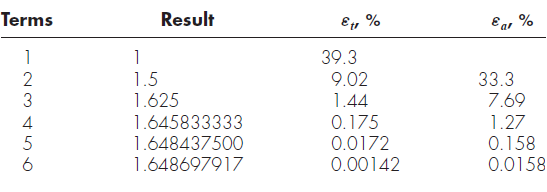
\includegraphics{./images/fig_4_1_1}
    \end{figure}

    \noindent
    Thus, after six terms are included, the approximate error falls below $\epsilon_s=0.05\%$, and the
    computation is terminated. However, notice that, rather than three significant figures, the
    result is accurate to five! This is because, for this case, both Eqs. (4.5) and (4.7) are conservative.
    That is, they ensure that the result is at least as good as they specify. Although,
    this is not always the case for Eq. (4.5), it is true most of the time.\\
\end{example}

\subsection{Computer Algorithm for Iterative Calculations}

\noindent
Many of the numerical methods described in the remainder of this text involve iterative
calculations of the sort illustrated in Example 4.1. These all entail solving a mathematical
problem by computing successive approximations to the solution starting from an initial
guess.

The computer implementation of such iterative solutions involves loops. As we saw in
Sec. 3.3.2, these come in two basic flavors: count-controlled and decision loops. Most iterative
solutions use decision loops. Thus, rather than employing a pre-specified number of
iterations, the process typically is repeated until an approximate error estimate falls below
a stopping criterion as in Example 4.1.

To do this for the same problem as Example 4.1, the series expansion can be expressed
as
\newline

$e^x\cong \mathlarger{\sum}_{i=0}^{n}\dfrac{x^n}{n!}$
\newline

\noindent
An M-file to implement this formula is shown in Fig. 4.2. The function is passed the value
to be evaluated (\texttt{x}) along with a stopping error criterion (\texttt{es}) and a maximum allowable
number of iterations (\texttt{maxit}). If the user omits either of the latter two parameters, the function
assigns default values.
\newline

\begin{figure}[h]
    \begin{lstlisting}[numbers=none]
 function [fx, ea, iter] = IterMeth(x,es,maxit)
 % Maclaurin series of exponential function
 %   [fx,ea,iter] = IterMeth(x,es,maxit)
 % input:
 %   x = value at which series evaluated
 %   es = stopping criterion (default = 0.0001)
 %   maxit = maximum iterations (default = 50)
 % output:
 %   fx = estimated value
 %   ea = approximate relative error (%)
 %   iter = number of iterations    
 % defaults:
 if nargin<2|isempty(es), es=0.0001; end
 if nargin<3|isempty(maxit), maxit=50; end
 % initialization
 iter = 1; sol = 1; ea = 100;
 % iterative calculation
 while (1)
     solold = sol;
     sol = sol + x ^ iter / factorial(iter);
     iter = iter + 1;
     if sol~=0
         ea=abs((sol - solold)/sol)*100;
     end
     if ea<=es | iter>=maxit,break,end
 end
 fx = sol
 end
    \end{lstlisting}
    \caption{An M-file to solve an iterative calculation. This example is set up to evaluate the Maclaurin series
    expansion for ex as described in Example 4.1.}
\end{figure}

The function then initializes three variables: \emph{(a)} \texttt{iter}, which keeps track of the number
of iterations, \emph{(b)} \texttt{sol}, which holds the current estimate of the solution, and \emph{(c)} a variable,
\texttt{ea}, which holds the approximate percent relative error. Note that \emph{ea} is initially set to a value
of 100 to ensure that the loop executes at least once.

These initializations are followed by a decision loop that actually implements the
iterative calculation. Prior to generating a new solution, the previous value, \texttt{sol}, is first assigned
to \texttt{solold}. Then a new value of \texttt{sol} is computed and the iteration counter is incremented.
If the new value of \texttt{sol} is nonzero, the percent relative error, \texttt{ea}, is determined.
The stopping criteria are then tested. If both are false, the loop repeats. If either is
true, the loop terminates and the final solution is sent back to the function call.

When the M-file is implemented, it generates an estimate for the exponential function
which is returned along with the approximate error and the number of iterations. For
example, $e^1$ can be evaluated as\\

\texttt{>> format long\\
\indent>> [approxval, ea, iter] = IterMeth(1,1e-6,100)\\
\indent approxval =\\ 
\indent\indent 2.718281826198493\\
\indent ea =\\
\indent\indent 9.216155641522974e-007\\
\indent iter =\\
\indent\indent 12}\\

We can see that after 12 iterations, we obtain a result of 2.7182818 with an
approximate error estimate of $= 9.2162 \times 10^{-7}\%$. The result can be verified by using
the built-in \texttt{exp} function to directly calculate the exact value and the true percent relative
error,\\

\texttt{>> trueval=exp(1)\\
\indent trueval =\\
\indent\indent 2.718281828459046\\
\indent >> et=abs((trueval- approxval)/trueval)*100\\
\indent et =\\
\indent\indent 8.316108397236229e-008}\\
    
\noindent
As was the case with Example 4.1, we obtain the desirable outcome that the true error is
less than the approximate error.
\vspace{10 mm}

\section{ROUNDOFF ERRORS}
\emph{Roundoff errors} arise because digital computers cannot represent some quantities exactly.
They are important to engineering and scientific problem solving because they
can lead to erroneous results. In certain cases, they can actually lead to a calculation
going unstable and yielding obviously erroneous results. Such calculations are said to
be \emph{ill-conditioned}. Worse still, they can lead to subtler discrepancies that are difficult
to detect.

There are two major facets of roundoff errors involved in numerical calculations:

\begin{enumerate}
    \item Digital computers have magnitude and precision limits on their ability to represent
    numbers.
    \item Certain numerical manipulations are highly sensitive to roundoff errors. This can result
    from both mathematical considerations as well as from the way in which computers
    perform arithmetic operations.
\end{enumerate}

\subsection{Computer Number Representation}
Numerical roundoff errors are directly related to the manner in which numbers are stored
in a computer. The fundamental unit whereby information is represented is called a \emph{word}.
This is an entity that consists of a string of binary \emph{digits}, or \emph{bits}. Numbers are typically
stored in one or more words. To understand how this is accomplished, we must first review
some material related to number systems.

A \emph{number system} is merely a convention for representing quantities. Because we have
10 fingers and 10 toes, the number system that we are most familiar with is the \emph{decimal}, or
\emph{base-10}, number system. A base is the number used as the reference for constructing the
system. The base-10 system uses the 10 digits---0, 1, 2, 3, 4, 5, 6, 7, 8, and 9---to represent
numbers. By themselves, these digits are satisfactory for counting from 0 to 9.

For larger quantities, combinations of these basic digits are used, with the position or
\emph{place value} specifying the magnitude. The rightmost digit in a whole number represents a
number from 0 to 9. The second digit from the right represents a multiple of 10. The third
digit from the right represents a multiple of 100 and so on. For example, if we have the
number 8642.9, then we have eight groups of 1000, six groups of 100, four groups of 10,
two groups of 1, and nine groups of 0.1, or\\

$(8 \times 10^3) + (6 \times 10^2) + (4 \times 10^1) + (2 \times 10^0) + (9 \times 10^{-1}) = 8642.9$\\

\noindent
This type of representation is called \emph{positional notation}.

Now, because the decimal system is so familiar, it is not commonly realized that
there are alternatives. For example, if human beings happened to have eight fingers and
toes we would undoubtedly have developed an \emph{octal}, or \emph{base-8}, representation. In the
same sense, our friend the computer is like a two-fingered animal who is limited to two
states---either 0 or 1. This relates to the fact that the primary logic units of digital computers
are on/off electronic components. Hence, numbers on the computer are represented
with a \emph{binary}, or \emph{base-2}, system. Just as with the decimal system, quantities
can be represented using positional notation. For example, the binary number 101.1 is
equivalent to $(1 \times 2^2)+(0 \times 2^1) + (1 \times 2^0) + (1 \times 2^{-1}) = 4 + 0 + 1 + 0.5 = 5.5$ in the
decimal system.\\

\noindent
\textbf{Integer Representation.}\quad
Now that we have reviewed how base-10 numbers can be represented
in binary form, it is simple to conceive of how integers are represented on a computer.
The most straightforward approach, called the \emph{signed magnitude method}, employs
the first bit of a word to indicate the sign, with a 0 for positive and a 1 for negative. The remaining
bits are used to store the number. For example, the integer value of 173 is represented
in binary as 10101101:\\

$(10101101)_2= 2^7 + 2^5 + 2^3 + 2^2 + 2^0 = 128 + 32 + 8 + 4 + 1 = (173)_{10}$\\

\noindent
Therefore, the binary equivalent of --173 would be stored on a 16-bit computer, as depicted
in Fig. 4.3.

If such a scheme is employed, there clearly is a limited range of integers that can be represented.
Again assuming a 16-bit word size, if one bit is used for the sign, the 15 remaining
bits can represent binary integers from 0 to 111111111111111. The upper limit can be converted
to a decimal integer, as in 

$(1 \times2^{14}) +(1 \times2^{13}) +\hdots +(1 \times2^{1}) +(1 \times2^{0}) = 32,767$.\\


\begin{figure}[h]
    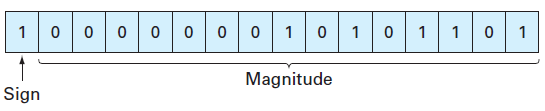
\includegraphics{./images/fig_4_3}
    \caption{The binary representation of the decimal integer -173 on a 16-bit computer using the signed
    magnitude method.}
\end{figure}

\noindent
Note that this value can be simply evaluated as $2^{15}-1$. Thus, a 16-bit computer word can
store decimal integers ranging from --32,767 to 32,767.

In addition, because zero is already defined as 0000000000000000, it is redundant
to use the number \\1000000000000000 to define a ``minus zero''. Therefore, it is conventionally
employed to represent an additional negative number: --32,768, and the range is
from --32,768 to 32,767. For an n-bit word, the range would be from  $-2^{n-1}$ to $2^{n-1}-1$.
Thus, 32-bit integers would range from --2,147,483,648 to +2,147,483,647.

Note that, although it provides a nice way to illustrate our point, the signed magnitude
method is not actually used to represent integers for conventional computers. A preferred
approach called the 2s \emph{complement} technique directly incorporates the sign into the
number's magnitude rather than providing a separate bit to represent plus or minus.
Regardless, the range of numbers is still the same as for the signed magnitude method
described above.

The foregoing serves to illustrate how all digital computers are limited in their capability
to represent integers. That is, numbers above or below the range cannot be represented. A
more serious limitation is encountered in the storage and manipulation of fractional quantities
as described next.\\

\noindent
\textbf{Floating-Point Representation.}\quad Fractional quantities are typically represented in computers
using \emph{floating-point format}. In this approach, which is very much like scientific
notation, the number is expressed as\\

$\pm s\times b^e$\\

\noindent
where s = the \emph{significand} (or \emph{mantissa}), b = the base of the number system being used, and
e = the exponent.

Prior to being expressed in this form, the number is \emph{normalize}d by moving the decimal
place over so that only one significant digit is to the left of the decimal point. This is done so
computer memory is not wasted on storing useless nonsignificant zeros. For example, a value
like 0.005678 could be represented in a wasteful manner as $0.005678 \times 10^0$. However, normalization
would yield $5.678 \times 10^{-3}$ which eliminates the useless zeroes.

Before describing the base-2 implementation used on computers, we will first explore
the fundamental implications of such floating-point representation. In particular,
what are the ramifications of the fact that in order to be stored in the computer, both
the mantissa and the exponent must be limited to a finite number of bits? As in the
next example, a nice way to do this is within the context of our more familiar base-10
decimal world.\\

\begin{example} Implications of Floating-Point Representation
    \bigskip
    \newline
    \textbf{Problem Statement.}\quad Suppose that we had a hypothetical base-10 computer with a 5-digit
    word size. Assume that one digit is used for the sign, two for the exponent, and two for the
    mantissa. For simplicity, assume that one of the exponent digits is used for its sign, leaving
    a single digit for its magnitude.\\

    \noindent
    \textbf{Solution.}\quad A general representation of the number following normalization would be\\

    $s_1 d_1 d_2 \times 10^{s_0 d_0}$\\

    \noindent
    where $s_0$ and $s_1$ = the signs, $d_0$ = the magnitude of the exponent, and $d_1$ and $d_2$ = the magnitude
    of the significand digits.

    Now, let's play with this system. First, what is the largest possible positive quantity
    that can be represented? Clearly, it would correspond to both signs being positive and all
    magnitude digits set to the largest possible value in \\base-10, that is, 9:\\

    Largest value = $+9.9\times10^{+9}$\\

    \noindent
    So the largest possible number would be a little less than 10 billion. Although this might
    seem like a big number, it's really not that big. For example, this computer would be incapable
    of representing a commonly used constant like Avogadro's number $(6.022 \times 1023)$.
    In the same sense, the smallest possible positive number would be\\

    Smallest value = $+1.0 \times 10^{-9}$\\

    \noindent
    Again, although this value might seem pretty small, you could not use it to represent a
    quantity like Planck's constant $(6.626 \times 10^{-34} J \cdot s)$.
    
    Similar negative values could also be developed. The resulting ranges are displayed in
    Fig. 4.4. Large positive and negative numbers that fall outside the range would cause an
    overflow error. In a similar sense, for very small quantities there is a ``hole'' at zero, and
    very small quantities would usually be converted to zero.
    
    Recognize that the exponent overwhelmingly determines these range limitations. For
    example, if we increase the mantissa by one digit, the maximum value increases slightly to
    $9.99\times 10^9$. In contrast, a one-digit increase in the exponent raises the maximum by 90 orders
    of magnitude to $9.9\times 10^{99}$!
    
    When it comes to precision, however, the situation is reversed. Whereas the significand
    plays a minor role in defining the range, it has a profound effect on specifying the precision.
    This is dramatically illustrated for this example where we have limited the significand to
    only 2 digits. As in Fig. 4.5, just as there is a ``hole'' at zero, there are also ``holes'' between
    values.
    
    For example, a simple rational number with a finite number of digits like $2^{-5} = 0.03125$
    would have to be stored as $3.1 \times 10{−2}$ or 0.031. Thus, a \emph{roundoff error} is introduced. For this
    case, it represents a relative error of\\

    $\dfrac{0.03125-0.031}{0.03125}=0.008$\\

    \begin{figure}[h]
        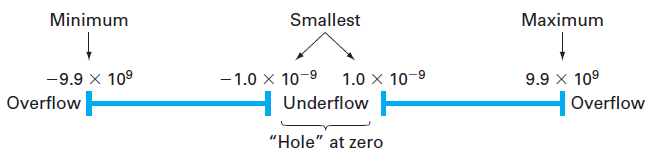
\includegraphics{./images/fig_4_4}
        \caption{The number line showing the possible ranges corresponding to the hypothetical base-10
        floating-point scheme described in Example 4.2.}
    \end{figure}

    \begin{figure}[h]
        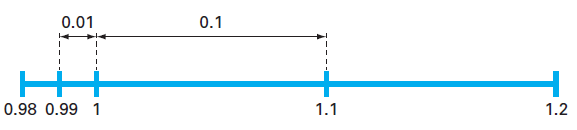
\includegraphics{./images/fig_4_5}
        \caption{A small portion of the number line corresponding to the hypothetical base-10 floating-point
        scheme described in Example 4.2. The numbers indicate values that can be represented
        exactly. All other quantities falling in the ``holes'' between these values would exhibit some
        roundoff error.}
    \end{figure}

    While we could store a number like 0.03125 exactly by expanding the digits of the
    significand, quantities with infinite digits must always be approximated. For example, a
    commonly used constant such as $\pi (=3.14159\hdots)$ would have to be represented as $3.1\times 10^0$
    or 3.1. For this case, the relative error is\\

    $\dfrac{3.14159-3.1}{3.14159} = 0.0132$\\

    \noindent
    Although adding significand digits can improve the approximation, such quantities will
    always have some roundoff error when stored in a computer.
    
    Another more subtle effect of floating-point representation is illustrated by Fig. 4.5.
    Notice how the interval between numbers increases as we move between orders of magnitude.
    For numbers with an exponent of --1 (i.e., between 0.1 and 1), the spacing is 0.01.
    Once we cross over into the range from 1 to 10, the spacing increases to 0.1. This means
    that the roundoff error of a number will be proportional to its magnitude. In addition, it
    means that the relative error will have an upper bound. For this example, the maximum
    relative error would be 0.05. This value is called the \emph{machine epsilon} (or machine
    precision).\\
\end{example}

As illustrated in Example 4.2, the fact that both the exponent and significand are finite
means that there are both range and precision limits on floating-point representation. Now,
let us examine how floating-point quantities are actually represented in a real computer
using base-2 or binary numbers.

First, let's look at normalization. Since binary numbers consist exclusively of 0s and
1s, a bonus occurs when they are normalized. That is, the bit to the left of the binary point
will always be one! This means that this leading bit does not have to be stored. Hence,
nonzero binary floating-point numbers can be expressed as\\

$\pm (1+f)\times 2^e$\\

\noindent
where f = the \emph{mantissa} (i.e., the fractional part of the significand). For example, if we normalized
the binary number 1101.1, the result would be $1.1011\times (2)^{-3}$ or $(1+0.1011)\times2^{-3}$.

\begin{figure}[h]
    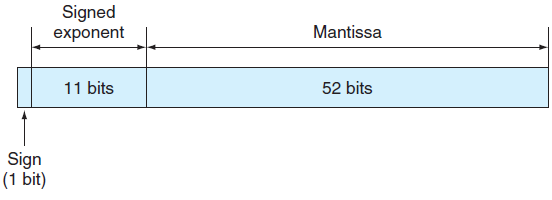
\includegraphics{./images/fig_4_6}
    \caption{The manner in which a floating-point number is stored in an 8-byte word in IEEE doubleprecision
    format.}
\end{figure}

\noindent
Thus, although the original number has five significant bits, we only have to store the four
fractional bits: 0.1011.

By default, MATLAB has adopted the \emph{IEEE double-precision format} in which eight
bytes (64 bits) are used to represent floating-point numbers. As in Fig. 4.6, one bit is reserved
for the number's sign. In a similar spirit to the way in which integers are stored, the
exponent and its sign are stored in 11 bits. Finally, 52 bits are set aside for the mantissa.
However, because of normalization, 53 bits can be stored.

Now, just as in Example 4.2, this means that the numbers will have a limited range and
precision. However, because the IEEE format uses many more bits, the resulting number
system can be used for practical purposes.\\

\noindent
\textbf{Range}\quad In a fashion similar to the way in which integers are stored, the 11 bits used for
the exponent translates into a range from --1022 to 1023. The largest positive number can
be represented in binary as\\

Largest value = $+1.1111\hdots1111\times 2^{+1023}$\\

\noindent
where the 52 bits in the mantissa are all 1. Since the significant is approximately 2 (it is
actually $2-2^{-52}$), the largest value is therefore $2^{1024}=1.7977\times 10^{308}$. In a similar
fashion, the smallest positive number can be represented as\\

Smallest value = $+1.0000\hdots 0000\times 2^{-1022}$\\

\noindent
This value can be translated into a base-10 value of $2^{-1022}=2.2251\times10^{-308}$\\

\noindent
\textbf{Precision.}\quad The 52 bits used for the mantissa correspond to about 15 to 16 base-10 digits.
Thus, $\pi$ would be expressed as

\texttt{>> format long\\
\indent >> pi\\
\indent ans =\\
\indent\indent 3.14159265358979}\\

\noindent
Note that the machine epsilon is $2^{-52}=2.2204\times 10^{-16}$\\

MATLAB has a number of built-in functions related to its internal number representation.
For example, the \texttt{realmax} function displays the largest positive real number:\\

\texttt{>> format long\\
\indent >> realmax\\
\indent ans =\\
\indent\indent 1.797693134862316e+308}\\

Numbers occurring in computations that exceed this value create an overflow. In MATLAB
they are set to infinity, \texttt{inf}. The \texttt{realmin} function displays the smallest positive real
number:\\

\texttt{>> realmin\\
\indent ans =\\
\indent\indent 2.225073858507201e-308}\\

\noindent
Numbers that are smaller than this value create an \emph{underflow} and, in MATLAB, are set to
zero. Finally, the \texttt{eps} function displays the machine epsilon:\\

\texttt{>> eps\\
\indent ans=\\
\indent\indent 2.220446049250313e-016}\\

\subsection{Arithmetic Manipulations of Computer Numbers}

\noindent
Aside from the limitations of a computer's number system, the actual arithmetic manipulations
involving these numbers can also result in roundoff error. To understand how this
occurs, let's look at how the computer performs simple addition and subtraction.

Because of their familiarity, normalized base-10 numbers will be employed to illustrate
the effect of roundoff errors on simple addition and subtraction. Other number bases
would behave in a similar fashion. To simplify the discussion, we will employ a hypothetical
decimal computer with a 4-digit mantissa and a 1-digit exponent.

When two floating-point numbers are added, the numbers are first expressed so that
they have the same exponents. For example, if we want to add $1.557 + 0.04341$, the computer
would express the numbers as \\$0.1557\times 10^1 + 0.004341\times 10^1$. Then the mantissas
are added to give $0.160041 \times 10^1$. Now, because this hypothetical computer only carries a
4-digit mantissa, the excess number of digits get chopped off and the result is $0.1600\times 10^1$.
Notice how the last two digits of the second number (41) that were shifted to the right have
essentially been lost from the computation.

Subtraction is performed identically to addition except that the sign of the subtrahend
is reversed. For example, suppose that we are subtracting 26.86 from 36.41. That is,\\

\begin{tabular}{c c c}
        & $0.3641 \times 10^2$\\
    -   & $0.2686 \times 10^2$\\
        \hline
        & $0.0955 \times 10^2$\\
\end{tabular}\\

For this case the result must be normalized because the leading zero is unnecessary. So
we must shift the decimal one place to the right to give $0.9550 \times 10^1 = 9.550$. Notice that
the zero added to the end of the mantissa is not significant but is merely appended to fill the
empty space created by the shift. Even more dramatic results would be obtained when the
numbers are very close as in\\

\begin{tabular}{c c c}
    & $0.7642 \times 10^3$\\
-   & $0.7641 \times 10^3$\\
    \hline
    & $0.0001 \times 10^3$\\
\end{tabular}\\

\noindent
which would be converted to $0.1000 \times 10^0 = 0.1000$. Thus, for this case, three nonsignificant
zeros are appended.
The subtracting of two nearly equal numbers is called \emph{subtractive cancellation}. It is
the classic example of how the manner in which computers handle mathematics can lead to
numerical problems. Other calculations that can cause problems include:\\

\noindent
\textbf{Large Computations.}\quad Certain methods require extremely large numbers of arithmetic
manipulations to arrive at their final results. In addition, these computations are often interdependent.
That is, the later calculations are dependent on the results of earlier ones. Consequently,
even though an individual roundoff error could be small, the cumulative effect
over the course of a large computation can be significant. Avery simple case involves summing
a round base-10 number that is not round in base-2. Suppose that the following M-file
is constructed:\\

\texttt{function sout = sumdemo()\\
\indent s = 0;\\
\indent for i = 1:10000\\
\indent\hspace{5 mm} s = s + 0.0001;\\
\indent end\\
\indent sout = s;}\\

\noindent
When this function is executed, the result is

\texttt{>> format long\\
\indent >> sumdemo\\
\indent ans =\\
\indent\indent 0.99999999999991}\\

The \texttt{format long} command lets us see the 15 significant-digit representation used
by MATLAB. You would expect that sum would be equal to 1. However, although
0.0001 is a nice round number in base-10, it cannot be expressed exactly in base-2. Thus,
the sum comes out to be slightly different than 1. We should note that MATLAB has features
that are designed to minimize such errors. For example, suppose that you form a
vector as in\\

\texttt{>> format long\\
\indent s = [0:0.0001:1];}\\

\noindent
For this case, rather than being equal to 0.99999999999991, the last entry will be exactly
one as verified by

\texttt{>> s(10001)\\
\indent ans =\\
\indent\indent 1}\\

\noindent
\textbf{Adding a Large and a Small Number.}\quad Suppose we add a small number, 0.0010, to a
large number, 4000, using a hypothetical computer with the 4-digit mantissa and the 1-digit
exponent. After modifying the smaller number so that its exponent matches the larger,\\

\begin{tabular}{c c c}
    & $0.4000$\hspace{5.5mm} & $ \times 10^4$\\
    & $0.0000001$ & $ \times 10^4$\\
    \hline
    & $0.4000001$ & $ \times 10^4$\\
\end{tabular}\\

\noindent
which is chopped to $0.4000 \times 10^4$ . Thus, we might as well have not performed the addition!
This type of error can occur in the computation of an infinite series. The initial terms
in such series are often relatively large in comparison with the later terms. Thus, after a few
terms have been added, we are in the situation of adding a small quantity to a large quantity.
One way to mitigate this type of error is to sum the series in reverse order. In this way,
each new term will be of comparable magnitude to the accumulated sum.\\

\noindent
\textbf{Smearing.}\quad Smearing occurs whenever the individual terms in a summation are larger
than the summation itself. One case where this occurs is in a series of mixed signs.\\

\noindent
\textbf{Inner Products.}\quad As should be clear from the last sections, some infinite series are particularly
prone to roundoff error. Fortunately, the calculation of series is not one of the more
common operations in numerical methods. A far more ubiquitous manipulation is the calculation
of inner products as in\\

$\mathlarger{\sum}_{i=1}^{n}x_i y_i = x_1 y_1 + x_2 y_2 + \hdots + x_n y_n$\\

\noindent
This operation is very common, particularly in the solution of simultaneous linear algebraic
equations. Such summations are prone to roundoff error. Consequently, it is often desirable to
compute such summations in double precision as is done automatically in MATLAB.\\
\bigskip

\section[TRUNCATION ERRORS]{TRUNCATION ERRORS}
\noindent
\emph{Truncation errors} are those that result from using an approximation in place of an exact
mathematical procedure. For example, in Chap. 1 we approximated the derivative of velocity
of a bungee jumper by a finite-difference equation of the form [Eq. (1.11)]\\

$\dfrac{dv}{dt} \cong \dfrac{\Delta v}{\Delta t} = \dfrac{v(t_{i+1})-v(t_i)}{t_{i+1}-t_i}$
\hfill
(4.8)\\

\noindent
A truncation error was introduced into the numerical solution because the difference equation
only approximates the true value of the derivative (recall Fig. 1.3). To gain insight into
the properties of such errors, we now turn to a mathematical formulation that is used widely
in numerical methods to express functions in an approximate fashion---the Taylor series.\\

\subsection{The Taylor Series}
\noindent
Taylor's theorem and its associated formula, the Taylor series, is of great value in the study
of numerical methods. In essence, the \emph{Taylor theorem} states that any smooth function can
be approximated as a polynomial. The \emph{Taylor series} then provides a means to express this
idea mathematically in a form that can be used to generate practical results.\\
\bigskip

\begin{figure}[h]
    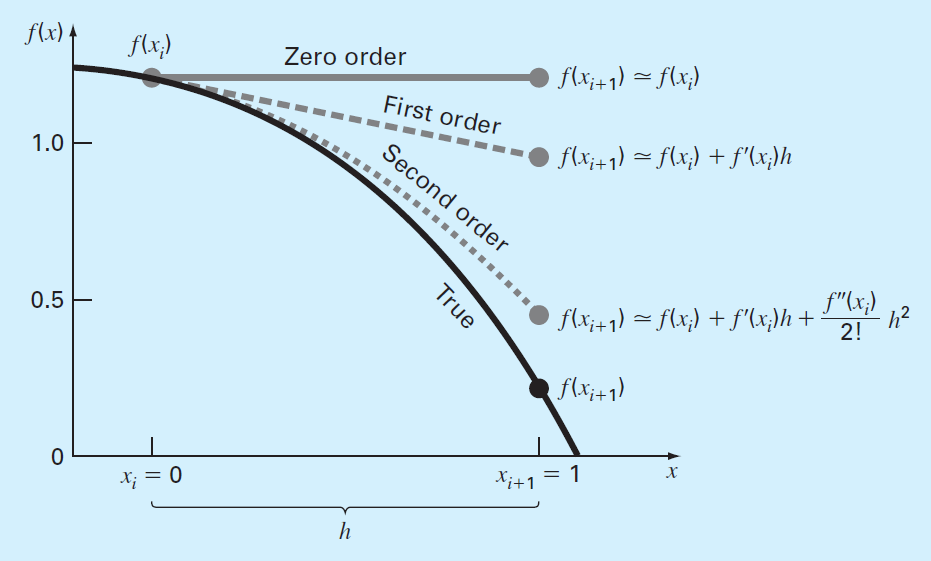
\includegraphics[width=0.8\linewidth]{./images/fig_4_7}
    \caption{The approximation of $f(x)=-0.1x^4 - 0.15x^3 - 0.5x^2 - 0.25x =1.2$ at $x = 1$ by
    zero-order, first-order, and second-order Taylor series expansions.}
\end{figure}
\bigskip

A useful way to gain insight into the Taylor series is to build it term by term. A good
problem context for this exercise is to predict a function value at one point in terms of the
function value and its derivatives at another point.

Suppose that you are blindfolded and taken to a location on the side of a hill facing
downslope (Fig. 4.7). We'll call your horizontal location $x_i$ and your vertical distance with
respect to the base of the hill $f(x_i)$. You are given the task of predicting the height at a
position $x_{i+1}$, which is a distance $h$ away from you.

At first, you are placed on a platform that is completely horizontal so that you have no
idea that the hill is sloping down away from you. At this point, what would be your best
guess at the height at $x_{i+1}$? If you think about it (remember you have no idea whatsoever
what's in front of you), the best guess would be the same height as where you're standing
now! You could express this prediction mathematically as\\

$f(x_{i+1}) \cong f(x_i)$
\hfill
(4.9)\\

\noindent
This relationship, which is called the \emph{zero-order approximation}, indicates that the value of
$f$ at the new point is the same as the value at the old point. This result makes intuitive sense
because if $x_i$ and $x_{i+1}$ are close to each other, it is likely that the new value is probably similar
to the old value.

Equation (4.9) provides a perfect estimate if the function being approximated is, in
fact, a constant. For our problem, you would be right only if you happened to be standing
on a perfectly flat plateau. However, if the function changes at all over the interval, additional
terms of the Taylor series are required to provide a better estimate.

So now you are allowed to get off the platform and stand on the hill surface with one
leg positioned in front of you and the other behind. You immediately sense that the front
foot is lower than the back foot. In fact, you're allowed to obtain a quantitative estimate of
the slope by measuring the difference in elevation and dividing it by the distance between
your feet.

With this additional information, you're clearly in a better position to predict the
height at $f(x_{i+1})$. In essence, you use the slope estimate to project a straight line out to
$x_{i+1}$. You can express this prediction mathematically by\\

$f(x_{i+1})\cong f(x_i)+f'(x_i)h$
\hfill
(4.10)\\

\noindent
This is called a \emph{first-order approximation} because the additional first-order term consists of
a slope $f'(x_i)$ multiplied by $h$, the distance between $x_i$ and $x_{i+1}$. Thus, the expression is
now in the form of a straight line that is capable of predicting an increase or decrease of the
function between $x_i$ and $x_{i+1}$.\\

Although Eq. (4.10) can predict a change, it is only exact for a straight-line, or \emph{linear},
trend. To get a better prediction, we need to add more terms to our equation. So now you
are allowed to stand on the hill surface and take two measurements. First, you measure the
slope behind you by keeping one foot planted at $x_i$ and moving the other one back a distance
$\Delta x$. Let's call this slope $f_b'(x_i)$. Then you measure the slope in front of you by keeping
one foot planted at $x_i$ and moving the other one forward $\Delta x$. Let's call this slope
$f_f'(x_i)$. You immediately recognize that the slope behind is milder than the one in front.
Clearly the drop in height is ``accelerating'' downward in front of you. Thus, the odds are
that $f(x_i)$ is even lower than your previous linear prediction.

As you might expect, you're now going to add a second-order term to your equation
and make it into a parabola. The Taylor series provides the correct way to do this as in\\

$f(x_{i+1})\cong f(x_i)+f'(x_i)h+\dfrac{f''(x_i)}{2!}h^2$
\hfill
(4.11)\\

\noindent
To make use of this formula, you need an estimate of the second derivative. You can use the
last two slopes you determined to estimate it as\\

$f''(x_{i+1})\cong\dfrac{f_f'(x_i)-f_b'(x_i)}{\Delta x}$
\hfill
(4.12)\\

\noindent
Thus, the second derivative is merely a derivative of a derivative; in this case, the rate of
change of the slope.

Before proceeding, let's look carefully at Eq. (4.11). Recognize that all the values
subscripted $i$ represent values that you have estimated. That is, they are numbers. Consequently,
the only unknowns are the values at the prediction position $x_{i+1}$. Thus, it is a quadratic
equation of the form\\

$f(h)\cong a_2h^2+a_1h+a_0$\\

\noindent
Thus, we can see that the second-orderTaylor series approximates the function with a secondorder
polynomial.

Clearly, we could keep adding more derivatives to capture more of the function’s curvature.
Thus, we arrive at the complete Taylor series expansion\\

$f(x_{i+1})=f(x_i) + f'(x_i)h + \dfrac{f''(x_i)}{2!}h^2 + \dfrac{f^{(3)}(x_i)}{3!}h^3 +
\hdots + \dfrac{f^{(n)}(x_i)}{n!}h^n + R_n$
\hfill
(4.13)\\

\noindent
Note that because Eq. (4.13) is an infinite series, an equal sign replaces the approximate
sign that was used in Eqs. (4.9) through (4.11). A remainder term is also included to
account for all terms from $n + 1$ to infinity:\\

$R_n = \dfrac{f^{(n+1)}(\xi)}{(n+1)!}h^{n+1}$
\hfill
(4.14)\\

\noindent
where the subscript $n$ connotes that this is the remainder for the $n$th-order approximation
and $\xi$ is a value of $x$ that lies somewhere between $x_i$ and $x_{i+1}$.

We can now see why the Taylor theorem states that any smooth function can be approximated
as a polynomial and that the Taylor series provides a means to express this idea
mathematically.

In general, the $n$th-order Taylor series expansion will be exact for an $n$th-order polynomial.
For other differentiable and continuous functions, such as exponentials and sinusoids,
a finite number of terms will not yield an exact estimate. Each additional term will
contribute some improvement, however slight, to the approximation. This behavior will be
demonstrated in Example 4.3. Only if an infinite number of terms are added will the series
yield an exact result.

Although the foregoing is true, the practical value of Taylor series expansions is that,
in most cases, the inclusion of only a few terms will result in an approximation that is close
enough to the true value for practical purposes. The assessment of how many terms are
required to get ``close enough'' is based on the remainder term of the expansion (Eq. 4.14).
This relationship has two major drawbacks. First, $\xi$ is not known exactly but merely lies
somewhere between $x_i$ and $x_{i+1}$. Second, to evaluate Eq. (4.14), we need to determine the
$(n + 1)$th derivative of $f (x)$. To do this, we need to know $f (x)$. However, if we knew
$f (x)$, there would be no need to perform the Taylor series expansion in the present
context!

Despite this dilemma, Eq. (4.14) is still useful for gaining insight into truncation
errors. This is because we \emph{do} have control over the term $h$ in the equation. In other words,
we can choose how far away from $x$ we want to evaluate $f (x)$, and we can control the number
of terms we include in the expansion. Consequently, Eq. (4.14) is often expressed as\\

$R_n=O(h^{n+1})$\\

\noindent
where the nomenclature $O(h^{n+1})$ means that the truncation error is of the order of $h^{n+1}$.
That is, the error is proportional to the step size $h$ raised to the $(n + 1)$th power. Although
this approximation implies nothing regarding the magnitude of the derivatives that multiply
$h^{n+1}$, it is extremely useful in judging the comparative error of numerical methods
based on Taylor series expansions. For example, if the error is $O(h)$, halving the step size
will halve the error. On the other hand, if the error is $O(h^2)$, halving the step size will quarter
the error.

In general, we can usually assume that the truncation error is decreased by the addition
of terms to the Taylor series. In many cases, if $h$ is sufficiently small, the first- and other
lower-order terms usually account for a disproportionately high percent of the error. Thus,
only a few terms are required to obtain an adequate approximation. This property is illustrated
by the following example.\\

\begin{example} Approximation of a Function with a Taylor Seres Expansion
    \bigskip\\
    \textbf{Problem Statement.}\quad Use Taylor series expansions with $n=0$ to 6 to approximate
    $f(x)=cos x$ at $x_{i+1} = \pi/3$ on the basis of the value of $f(x)$ and its derivatives
    at $x_i=\pi/4$. Note that this means that $h=\pi/3-\pi/4=\pi/12$.\\

    \noindent
    \textbf{Solution.}\quad Our knowledge of the true function allows us to determine the correct value
    $f (\pi/3) = 0.5$. The zero-order approximation is [Eq. (4.9)]\\

    $f\Big(\dfrac{\pi}{3}\Big)\cong cos\Big(\dfrac{\pi}{4}\Big)=0.707106781$\\

    \noindent
    which represents a percent relative error of\\

    $\epsilon_t = \left\lvert \dfrac{0.5-0.707106781}{0.5}\right\rvert100\%=41.1\% $\\

    \noindent
    For the first-order approximation, we add the first derivative term where $f'(x)=-sin x$:\\

    $f\Big(\dfrac{\pi}{3}\Big)\cong cos\Big(\dfrac{\pi}{4}\Big) - sin\Big(\dfrac{\pi}{4}\Big)\Big(\dfrac{\pi}{12}\Big) = 0.521986659$\\

    \noindent
    which has $\left\lvert\epsilon_t \right\rvert = 4.40\%$. For the second-order approximation, we add the second derivative
    term where $f''(x) = -cosx$:\\

    $f\Big(\dfrac{\pi}{3}\Big)\cong cos\Big(\dfrac{\pi}{4}\Big) - sin\Big(\dfrac{\pi}{4}\Big)\Big(\dfrac{\pi}{12}\Big) 
    -\dfrac{cos(\pi/4)}{2}\Big(\dfrac{\pi}{12}\Big)^2 = 0.497754491$\\

    \noindent
    with $\left\lvert\epsilon_t \right\rvert = 0.449\%$. Thus, the inclusion of additional terms results in an improved estimate.
    The process can be continued and the results listed as in\\

    \begin{figure}[h]
        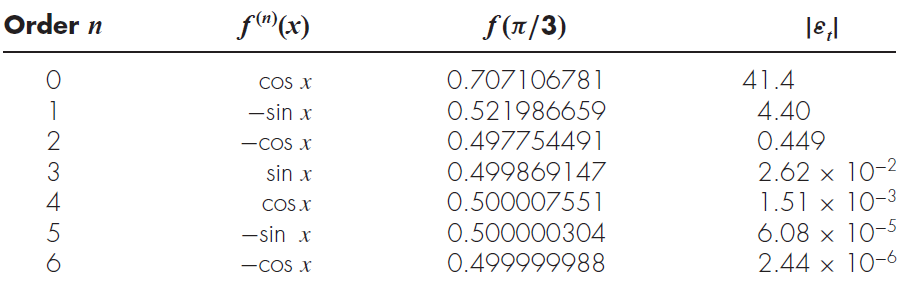
\includegraphics[width=0.8\linewidth]{./images/fig_7_1}
    \end{figure}

    Notice that the derivatives never go to zero as would be the case for a polynomial.
    Therefore, each additional term results in some improvement in the estimate. However,
    also notice how most of the improvement comes with the initial terms. For this case, by the
    time we have added the third-order term, the error is reduced to $0.026\%$, which means that
    we have attained $99.974\%$ of the true value. Consequently, although the addition of more
    terms will reduce the error further, the improvement becomes negligible.\\
\end{example}

\subsection{The Remainder for the Taylor Series Expansion}
\noindent
Before demonstrating how the Taylor series is actually used to estimate numerical errors,
we must explain why we included the argument $\xi$ in Eq. (4.14). To do this, we will use a
simple, visually based explanation.

\noindent
Suppose that we truncated the Taylor series expansion [Eq. (4.13)] after the zero-order
term to yield\\

$f(x_{i+1})\cong f(x_i)$\\

\noindent
A visual depiction of this zero-order prediction is shown in Fig. 4.8. The remainder, or
error, of this prediction, which is also shown in the illustration, consists of the infinite
series of terms that were truncated\\

$R_0 = f'(x_i)h + \dfrac{f''(x_1)}{2!}h^2 + \dfrac{f^{(3)}(x_i)}{3!}h^3\hdots$\\

\noindent
It is obviously inconvenient to deal with the remainder in this infinite series format. One
simplification might be to truncate the remainder itself, as in\\

$R_0\cong f'(x_i)h$
\hfill
(4.15)\\

\noindent
Although, as stated in the previous section, lower-order derivatives usually account for a
greater share of the remainder than the higher-order terms, this result is still inexact because
of the neglected second- and higher-order terms. This  ``inexactness'' is implied by the
approximate equality symbol ($\cong$) employed in Eq. (4.15).
An alternative simplification that transforms the approximation into an equivalence is
based on a graphical insight. As in Fig. 4.9, the \emph{derivative mean-value theorem} states that
if a function $f (x)$ and its first derivative are continuous over an interval from $x_i$ to $x_{i+1}$, then\\

\begin{figure}[h]
    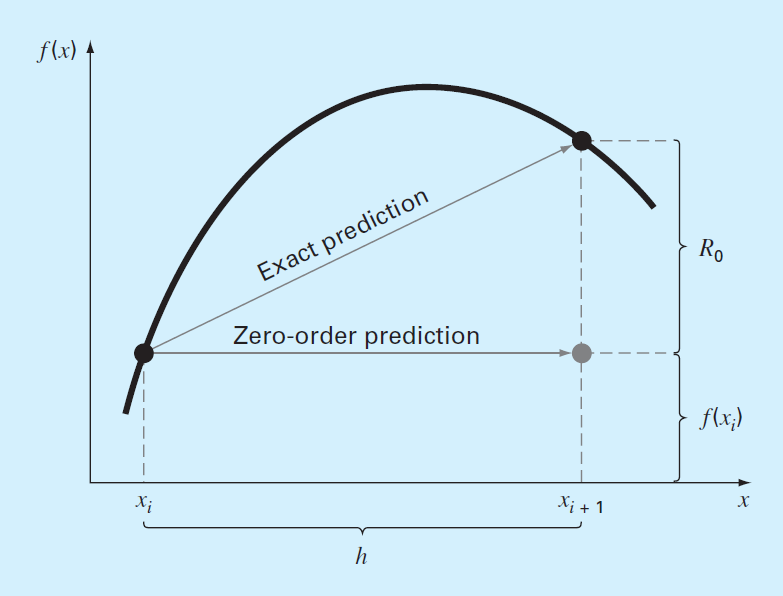
\includegraphics[width=0.55\linewidth]{./images/fig_4_8}
    \caption{Graphical depiction of a zero-order Taylor series prediction and remainder.\hfill}
\end{figure}

\begin{figure}[h]
    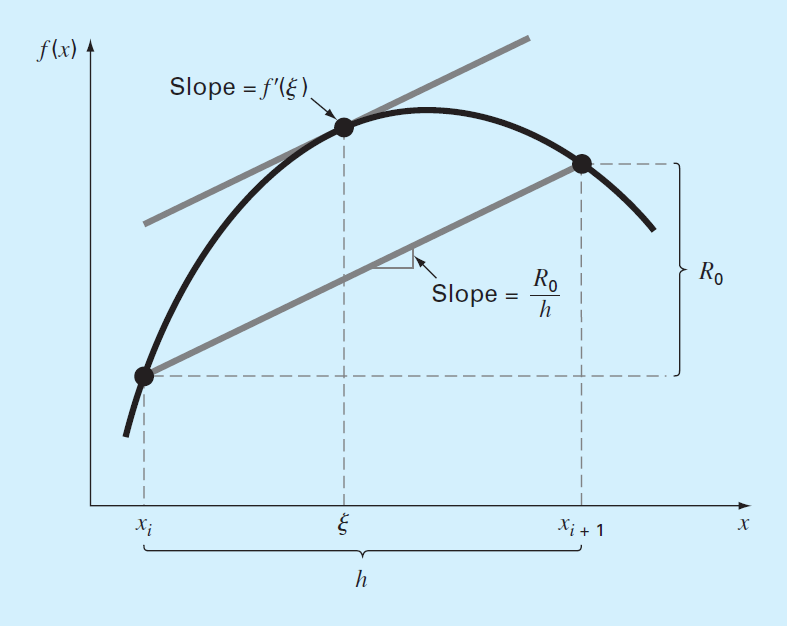
\includegraphics[width=0.55\linewidth]{./images/fig_4_9}
    \caption{Graphical depiction of the derivative mean-value theorem.}
\end{figure}

\noindent
there exists at least one point on the function that has a slope, designated by $f'(\xi)$, that is
parallel to the line joining $f(x_i)$ and $f(x_{i+1})$. The parameter $\xi$ marks the $x$ value where this
slope occurs (Fig. 4.9). A physical illustration of this theorem is that, if you travel between
two points with an average velocity, there will be at least one moment during the course of
the trip when you will be moving at that average velocity.
By invoking this theorem, it is simple to realize that, as illustrated in Fig. 4.9, the slope
$f'(\xi)$ is equal to the rise $R_0$ divided by the run $h$, or\\

$f'(\xi)=\dfrac{R_0}{h}$\\

\noindent
which can be rearranged to give\\

$R_0 = f'(\xi)h$
\hfill
(4.16)\\

\noindent
Thus, we have derived the zero-order version of Eq. (4.14). The higher-order versions
are merely a logical extension of the reasoning used to derive Eq. (4.16). The first-order
version is\\

$R_1 = \dfrac{f''(\xi)}{2!}h^2$
\hfill
(4.17)\\

\noindent
For this case, the value of $\xi$ conforms to the x value corresponding to the second derivative
that makes Eq. (4.17) exact. Similar higher-order versions can be developed from Eq. (4.14).\\

\subsection{Using the Taylor Series to Estimate Truncation Errors}
\noindent
Although the Taylor series will be extremely useful in estimating truncation errors throughout
this book, it may not be clear to you how the expansion can actually be applied to
numerical methods. In fact, we have already done so in our example of the bungee jumper.
Recall that the objective of both Examples 1.1 and 1.2 was to predict velocity as a function
of time. That is, we were interested in determining $v(t)$. As specified by Eq. (4.13), $v(t)$
can be expanded in a Taylor series:\\

$v(t_{i+1}) = v(t_i) + v'(t_i)(t_{i+1} - t_i) + \dfrac{v''(t_i)}{2!}(t_{i+1}-t_i)^2 + \hdots + R_n$\\

\noindent
Now let us truncate the series after the first derivative term:\\

$v(t_{i+1}) = v(t_i) + v'(t_i)(t_{i+1} - t_i) + R_1$
\hfill
(4.18)\\

\noindent
Equation (4.18) can be solved for\\

$v'(t_i) = \underbrace{\dfrac{v(t_{i+1})-v(t_i)}{t_{i+1}-t_i}}_\text{First-order approximation} - 
\underbrace{\dfrac{R_1}{t_{i+1}-t_i}}_\text{Truncation error}$
\hfill
(4.19)\\

\noindent
The first part of Eq. (4.19) is exactly the same relationship that was used to approximate
the derivative in Example 1.2 [Eq. (1.11)]. However, because of the Taylor series approach,
we have now obtained an estimate of the truncation error associated with this approximation
of the derivative. Using Eqs. (4.14) and (4.19) yields\\

$\dfrac{R_1}{t_{i+1}-t_i}=\dfrac{v''(\xi)}{2!}(t_{i+1}-t_i)$\\

\noindent
or\\

$\dfrac{R_1}{t_{i+1}-t_i}=O(t_{i+1}-t_i)$\\

\noindent
Thus, the estimate of the derivative [Eq. (1.11) or the first part of Eq. (4.19)] has a truncation
error of order $t_{i+1} - t_i$ . In other words, the error of our derivative approximation
should be proportional to the step size. Consequently, if we halve the step size, we would
expect to halve the error of the derivative.\\

\subsection{Numerical Differentiation}
\noindent
Equation (4.19) is given a formal label in numerical methods---it is called a \emph{finite difference}.
It can be represented generally as\\

$f'(x_i)=\dfrac{f(x_{i+1})-f(x_i)}{x_{i+1}-x_i} + O(x_{i+1}-x_i)$
\hfill
(4.20)\\

\noindent
or\\

$f'(x_i)=\dfrac{f(x_{i+1})-f(x_i)}{h} + O(h)$
\hfill
(4.21)\\

\noindent
where $h$ is called the step size---that is, the length of the interval over which the approximation
is made, $x_{i+1} - x_i$ . It is termed a ``forward'' difference because it utilizes data at $i$
and $i + 1$ to estimate the derivative (Fig. 4.10a).\\
\newpage

\begin{figure}[h]
    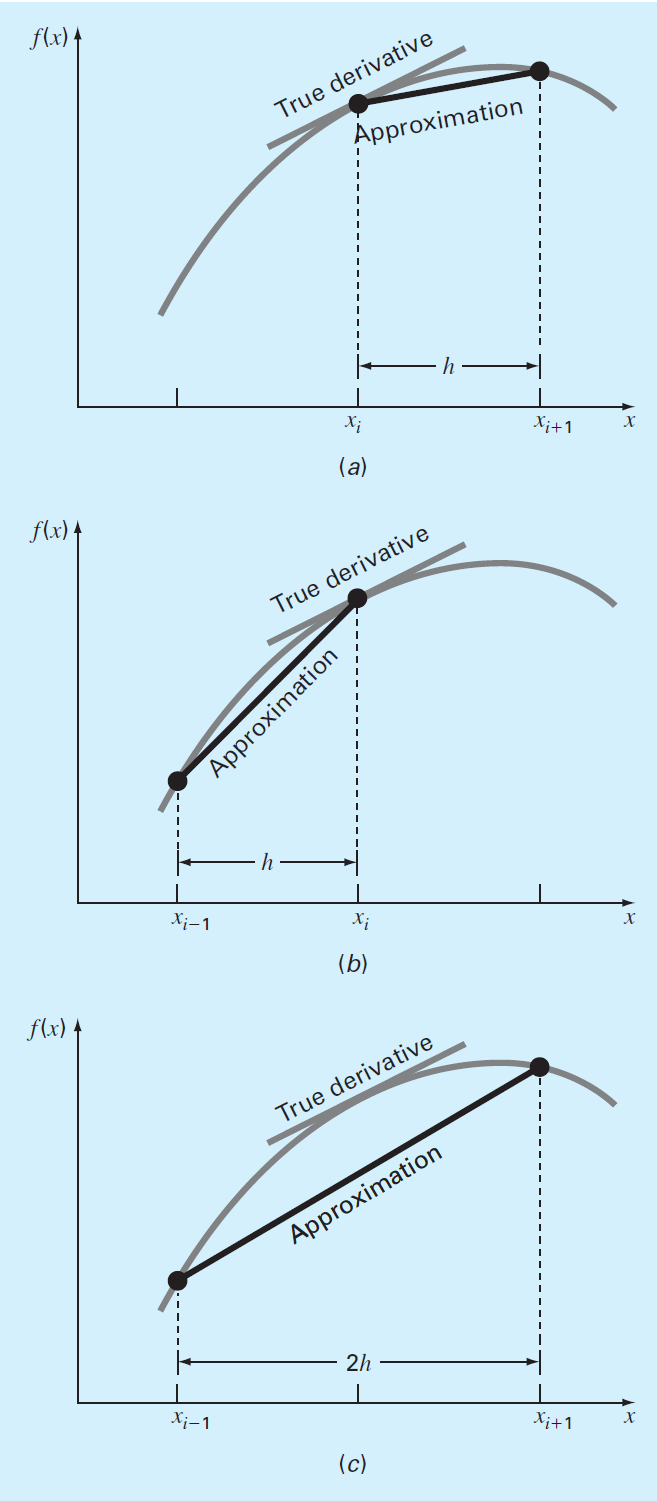
\includegraphics[width=0.5\linewidth]{./images/fig_4_10}
    \caption{Graphical depiction of (a) forward, (b) backward, and (c) centered finite-difference
    approximations of the first derivative.}
\end{figure}

This forward difference is but one of many that can be developed from the Taylor
series to approximate derivatives numerically. For example, backward and centered difference
approximations of the first derivative can be developed in a fashion similar to the
derivation of Eq. (4.19). The former utilizes values at $x_{i-1}$ and $x_i$ (Fig. 4.10b), whereas
the latter uses values that are equally spaced around the point at which the derivative is
estimated (Fig. 4.10c). More accurate approximations of the first derivative can be developed
by including higher-order terms of the Taylor series. Finally, all the foregoing versions
can also be developed for second, third, and higher derivatives. The following sections provide
brief summaries illustrating how some of these cases are derived.\\

\noindent\textbf{Backward Difference Approximation of the First Derivative.}\quad The Taylor series can be
expanded backward to calculate a previous value on the basis of a present value, as in\\

$f(x_{i-1}) = f(x_i)-f'(x_i)h+\dfrac{f''(x_i)}{2!}h^2-\hdots$
\hfill
(4.22)\\

\noindent
Truncating this equation after the first derivative and rearranging yields\\

$f'(x_i)\cong \dfrac{f(x_i)-f(x_{i-1})}{h}$
\hfill
(4.23)\\

\noindent
where the error is $O(h)$.\\

\noindent
\textbf{Centered Difference Approximation of the First Derivative.}\quad A third way to approximate
the first derivative is to subtract Eq. (4.22) from the forward Taylor series expansion:\\

$f(x_{i+1})=f(x_i)+f'(x_i)h + \dfrac{f''(x_i)}{2!}h^2 + \hdots$
\hfill
(4.24)\\

\noindent
to yield\\

$f(x_{i+1})=f(x_{i-1})+2f'(x_i)h + 2\dfrac{f^{(3)}(x_i)}{3!}h^3 + \hdots$\\

\noindent
which can be solved for\\

$f'(x_i)=\dfrac{f(x_{i+1})-f(x_{i-1})}{2h}-\dfrac{f^{(3)}(x_i)}{6}h^2+\hdots$\\

\noindent
or\\

$f'(x_i) = \dfrac{f(x_{i+1})-f(x_{i-1})}{2h}-O(h^2)$
\hfill
(4.25)\\

Equation (4.25) is a \emph{centered finite difference} representation of the first derivative.
Notice that the truncation error is of the order of $h^2$ in contrast to the forward and backward
approximations that were of the order of $h$. Consequently, the Taylor series analysis yields
the practical information that the centered difference is a more accurate representation of
the derivative (Fig. 4.10c). For example, if we halve the step size using a forward or backward
difference, we would approximately halve the truncation error, whereas for the central
difference, the error would be quartered.\\

\begin{example} Finite-Difference Approximations of Derivatives\\

    \noindent\textbf{Problem Statement.}\quad Use forward and backward difference approximations of $O(h)$ and
    a centered difference approximation of $O(h^2)$ to estimate the first derivative of\\

    $f(x) = -0.1x^4 - 0.15x^3 - 0.5x^2 - 0.25x + 1.2$\\

    \noindent
    at $x = 0.5$ using a step size $h = 0.5$. Repeat the computation using $h = 0.25$. Note that the
    derivative can be calculated directly as

    $f'(x) = -0.4x^3 - 0.45x^2 - 1.0x - 0.25$\\

    \noindent
    and can be used to compute the true value as $f'(0.5) = -0.9125$.\\

    \noindent
    \textbf{Solution.} \quad For $h = 0.5$, the function can be employed to determine\\

    $x_{i-1}=0$\hspace{10mm} $f(X_{i-1})=1.2$\\

    $x_i=0.5$ \hspace{9.8mm} $f(x_i) = 0.925$\\

    $x_{i+1}=1.0$\hspace{7.6mm} $f(x_{i+1}) = 0.2$\\

    \noindent
    These values can be used to compute the forward difference [Eq. (4.21)],\\

    $f'(0.5)\cong\dfrac{0.2-0.925}{0.5}=-1.45$\hspace{10mm} $\left\lvert\epsilon_t \right\rvert = 58.9\%$\\

    \noindent
    the backward difference [Eq. (4.23)],\\

    $f'(0.5)\cong\dfrac{0.925-1.2}{0.5}=-0.55$\hspace{10mm} $\left\lvert\epsilon_t \right\rvert = 39.7\%$\\

    \noindent
    and the centered difference [Eq. (4.25)],\\

    $f'(0.5)\cong\dfrac{0.2-1.2}{1.0}=-1.0$\hspace{10mm} $\left\lvert\epsilon_t \right\rvert = 9.6\%$\\

    \noindent
    For $h=0.25$,\\

    $x_{i-1}=0.25$\hspace{10mm} $f(x_{i-1})=1.10351563$\\

    $x_i=0.5$ \hspace{14mm} $f(x_i) = 0.925$\\

    $x_{i+1}=0.75$\hspace{10mm} $f(x_{i+1}) = 0.63632813$\\

    \noindent
    which can be used to compute the forward difference,\\

    $f'(0.5)\cong\dfrac{0.63632813 - 0.925}{0.25}=-1.155$\hspace{10mm} $\left\lvert\epsilon_t \right\rvert = 26.5\%$\\

    \noindent
    the backward difference,\\

    $f'(0.5)\cong\dfrac{0.925 - 1.10351563}{0.25}=-0.714$\hspace{10mm} $\left\lvert\epsilon_t \right\rvert = 21.7\%$\\

    \noindent
    and the centered difference,\\

    $f'(0.5)\cong\dfrac{0.63632813 - 1.10351563}{0.5}=-0.934$\hspace{10mm} $\left\lvert\epsilon_t \right\rvert = 2.4\%$\\


    For both step sizes, the centered difference approximation is more accurate than forward
    or backward differences. Also, as predicted by the Taylor series analysis, halving the
    step size approximately halves the error of the backward and forward differences and quarters
    the error of the centered difference.\\
\end{example}

\noindent
\textbf{Finite-Difference Approximations of Higher Derivatives.}\quad Besides first derivatives, the
Taylor series expansion can be used to derive numerical estimates of higher derivatives. To
do this, we write a forward Taylor series expansion for $f (x_{i+2})$ in terms of $f (x_i)$:\\

$f(x_{i+2})= f(x_i)+f'(x_i)(2h)+\dfrac{f''(x_i)}{2!}(2h)^2+\hdots$
\hfill
(4.26)\\

\noindent
Equation (4.24) can be multiplied by 2 and subtracted from Eq. (4.26) to give\\

$f(x_{i+2})-2f(x_{i+1})= -f(x_i)+f''(x_i)h^2+\hdots$\\

\noindent
which can be solved for\\

$f''(x_i)=\dfrac{f(x_{i+2})-2f(x_{i+1})+f(x_i)}{h^2}+O(h)$
\hfill
(4.27)\\

\noindent
This relationship is called the \emph{second forward finite difference}. Similar manipulations can
be employed to derive a backward version\\

$f''(x_i)=\dfrac{f(x_i)-2f(x_{i-1})+f(x_{i-2})}{h^2}+ O(h)$\\

\noindent
A centered difference approximation for the second derivative can be derived by
adding Eqs. (4.22) and (4.24) and rearranging the result to give\\

$f''(x_i)=\dfrac{f(x_{i+1})-2f(x_{i})+f(x_{i-1})}{h^2}+ O(h^2)$\\

\noindent
As was the case with the first-derivative approximations, the centered case is more accurate.
Notice also that the centered version can be alternatively expressed as\\

$f''(x_i)\cong \dfrac{\dfrac{f(x_{i+1})-f(x_i)}{h} - \dfrac{f(x_{i})-f(x_{i-1})}{h}}{h}$\\

\noindent
Thus, just as the second derivative is a derivative of a derivative, the second finite difference
approximation is a difference of two first finite differences [recall Eq. (4.12)].\\

\bigskip
\section[TOTAL NUMERICAL ERROR]{TOTAL NUMERICAL ERROR}

\noindent
The \emph{total numerical error} is the summation of the truncation and roundoff errors. In general,
the only way to minimize roundoff errors is to increase the number of significant figures
of the computer. Further, we have noted that roundoff error may \emph{increase} due to subtractive
cancellation or due to an increase in the number of computations in an analysis. In contrast,
Example 4.4 demonstrated that the truncation error can be reduced by decreasing the step
size. Because a decrease in step size can lead to subtractive cancellation or to an increase in
computations, the truncation errors are \emph{decreased} as the roundoff errors are \emph{increased}.\\

\begin{figure}[h]
    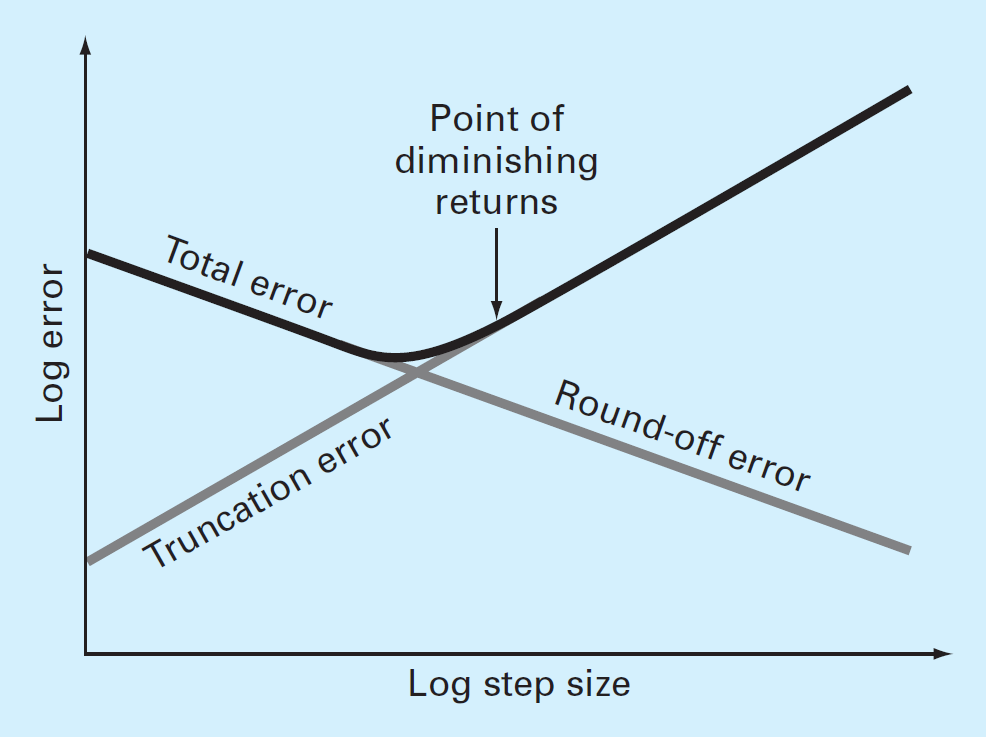
\includegraphics[width=0.6\linewidth]{./images/fig_4_11}
    \caption{A graphical depiction of the trade-off between roundoff and truncation error that sometimes
    comes into play in the course of a numerical method. The point of diminishing returns is
    shown, where roundoff error begins to negate the benefits of step-size reduction.}
\end{figure}

Therefore, we are faced by the following dilemma: The strategy for decreasing one
component of the total error leads to an increase of the other component. In a computation,
we could conceivably decrease the step size to minimize truncation errors only to discover
that in doing so, the roundoff error begins to dominate the solution and the total error
grows! Thus, our remedy becomes our problem (Fig. 4.11). One challenge that we face is
to determine an appropriate step size for a particular computation. We would like to choose
a large step size to decrease the amount of calculations and roundoff errors without incurring
the penalty of a large truncation error. If the total error is as shown in Fig. 4.11, the
challenge is to identify the point of diminishing returns where roundoff error begins to
negate the benefits of step-size reduction.
When using MATLAB, such situations are relatively uncommon because of its 15- to 16-
digit precision. Nevertheless, they sometimes do occur and suggest a sort of ``numerical uncertainty
principle'' that places an absolute limit on the accuracy that may be obtained using
certain computerized numerical methods. We explore such a case in the following section.\\

\subsection{Error Analysis of Numerical Differentiation}
\noindent
As described in Sec. 4.3.4, a centered difference approximation of the first derivative can
be written as (Eq. 4.25)\\

$\underset{\text{True value}}{f'(x_i)} = \underset{\text{Finite-difference approximation}}{\dfrac{f(x_{i+1})-f(x_{i-1})}{2h}}-\underset{\text{Truncation error}}{\dfrac{f^{(3)}(\xi)}{6}h^2}$
\hfill
(4.28)\\

\noindent
Thus, if the two function values in the numerator of the finite-difference approximation
have no roundoff error, the only error is due to truncation.

\noindent
However, because we are using digital computers, the function values do include
roundoff error as in\\

$f(x_{i-1}) = \tilde{f}(x_{i-1}) + e_{i-1}$\\

$f(x_{i+1}) = \tilde{f}(x_{i+1}) + e_{i+1}$\\

\noindent
where the $\tilde{f}$'s are the rounded function values and the e's are the associated roundoff
errors. Substituting these values into Eq. (4.28) gives\\

$\underset{\text{True value}}{f'(x_i)}=\underset{\text{Finite-difference approximation}}{\dfrac{\tilde{f}(x_{i+1})-\tilde{f}(x_{i-1})}{2h}}
 + \underset{\text{Roundoff error}}{\dfrac{e_{i+1}-e_{i-1}}{2h}}-\underset{\text{Truncation error}}{\dfrac{f^{(3)}(\xi)}{6}h^2}$\\

 \noindent
 We can see that the total error of the finite-difference approximation consists of a roundoff
error that decreases with step size and a truncation error that increases with step size.
Assuming that the absolute value of each component of the roundoff error has an
upper bound of $\epsilon$, the maximum possible value of the difference $e_{i+1} - e_{i-1}$ will be $2\epsilon$. Further,
assume that the third derivative has a maximum absolute value of $M$. An upper bound
on the absolute value of the total error can therefore be represented as\\

Total error = $\left\lvert f'(x_i)-\dfrac{\tilde{f}(x_{i+1})-\tilde{f}(x_{i-1})}{2h} \right\rvert \leq \dfrac{\epsilon}{h} + \dfrac{h^2M}{6}$
\hfill
(4.29)\\

\noindent
An optimal step size can be determined by differentiating Eq. (4.29), setting the result
equal to zero and solving for\\

$h_{opt}=\sqrt[3]{\dfrac{3\epsilon}{M}}$
\hfill
(4.30)\\

\begin{example} Roundoff and Truncation Errors in Numerical Differentiation\\

    \noindent\textbf{Problem Statement.}\quad In Example 4.4, we used a centered difference approximation of
    $O(h^2)$ to estimate the first derivative of the following function at $x = 0.5$,\\

    $f(x) = -0.1x^4 - 0.15x^3 - 0.5x^2 -0.25x + 1.2$\\

    \noindent
    Perform the same computation starting with $h = 1$. Then progressively divide the step size
    by a factor of 10 to demonstrate how roundoff becomes dominant as the step size is reduced.
    Relate your results to Eq. (4.30). Recall that the true value of the derivative is -0.9125.\\

    \noindent
    \textbf{Solution.} We can develop the following M-file to perform the computations and plot the
    results. Notice that we pass both the function and its analytical derivative as arguments:\\
    \texttt{\noindent 
    function diffex(func,dfunc,x,n)\\
    format long\\
    dftrue=dfunc(x);\\
    h=1;\\
    H(1)=h;\\
    D(1)=(func(x+h)-func(x-h))/(2*h);\\
    E(1)=abs(dftrue-D(1));\\
    for i=2:n\\
    \indent h=h/10;\\
    \indent H(i)=h;\\
    \indent D(i)=(func(x+h)-func(x-h))/(2*h);\\
    \indent E(i)=abs(dftrue-D(i));\\
    end\\
    L=[H' D' E']';\\
    fprintf(' step size finite difference true error\textbackslash n');\\
    fprintf('\%14.10f \%16.14f \%16.13f $\backslash$n', L);\\
    loglog(H, E), xlabel('Step Size'), ylabel('Error')\\
    title('Plot of Error Versus Step Size')\\
    format short\\}

    \noindent
    The M-file can then be run using the following commands:\\
  
    \texttt{\noindent >> ff=@(x) -0.1*x$\textasciicircum$4-0.15*x$\textasciicircum$3-0.5*x$\textasciicircum$2-0.25*x+1.2;}
  
    \texttt{\noindent >> df=@(x) -0.4*x$\textasciicircum$3-0.45*x$\textasciicircum$2-x-0.25;}
  
    \texttt{\noindent >> diffex(ff,df,0.5,11)}\\
    

\begin{tabular}{c c c}
    \texttt{step size} & \texttt{finite difference} & \texttt{true error}\\
    \texttt{1.0000000000} & \texttt{-1.26250000000000} & \texttt{0.3500000000000}\\
    \texttt{0.1000000000} & \texttt{-0.91600000000000} & \texttt{0.0035000000000}\\
    \texttt{0.0100000000} & \texttt{-0.91253500000000} & \texttt{0.0000350000000}\\
    \texttt{0.0010000000} & \texttt{-0.91250035000001} & \texttt{0.0000003500000}\\
    \texttt{0.0001000000} & \texttt{-0.91250000349985} & \texttt{0.0000000034998}\\
    \texttt{0.0000100000} & \texttt{-0.91250000003318} & \texttt{0.0000000000332}\\
    \texttt{0.0000010000} & \texttt{-0.91250000000542} & \texttt{0.0000000000054}\\
    \texttt{0.0000001000} & \texttt{-0.91249999945031} & \texttt{0.0000000005497}\\
    \texttt{0.0000000100} & \texttt{-0.91250000333609} & \texttt{0.0000000033361}\\
    \texttt{0.0000000010} & \texttt{-0.91250001998944} & \texttt{0.0000000199894}\\
    \texttt{0.0000000001} & \texttt{-0.91250007550059} & \texttt{0.0000000755006}
\end{tabular}\\
\bigskip

    As depicted in Fig. 4.12, the results are as expected. At first, roundoff is minimal and the
    estimate is dominated by truncation error. Hence, as in Eq. (4.29), the total error drops by a factor
    of 100 each time we divide the step by 10. However, starting at about $h = 0.0001$, we see
    roundoff error begin to creep in and erode the rate at which the error diminishes. A minimum
    error is reached at $h = 10^{-6}$. Beyond this point, the error increases as roundoff dominates.
    
    Because we are dealing with an easily differentiable function, we can also investigate
    whether these results are consistent with Eq. (4.30). First, we can estimate $M$ by evaluating
    the function's third derivative as\\

    $M = \left\lvert f^{(3)}(0.5) \right\rvert =  \left\lvert -2.4(0.5) - 0.9 \right\rvert = 2.1$\\

    \noindent
    Because MATLAB has a precision of about 15 to 16 base-10 digits, a rough estimate of the
    upper bound on roundoff would be about $\epsilon = 0.5 \times 10^{-16}$. Substituting these values into
    Eq. (4.30) gives\\

    $h_{opt} = \sqrt[3]{\dfrac{3(0.5\times 10^{-16})}{2.1}} = 4.3\times 10^{-6}$\\

    \noindent
    which is on the same order as the result of $1\times 10^{-6}$ obtained with MATLAB.\\

    \begin{figure}[h]
        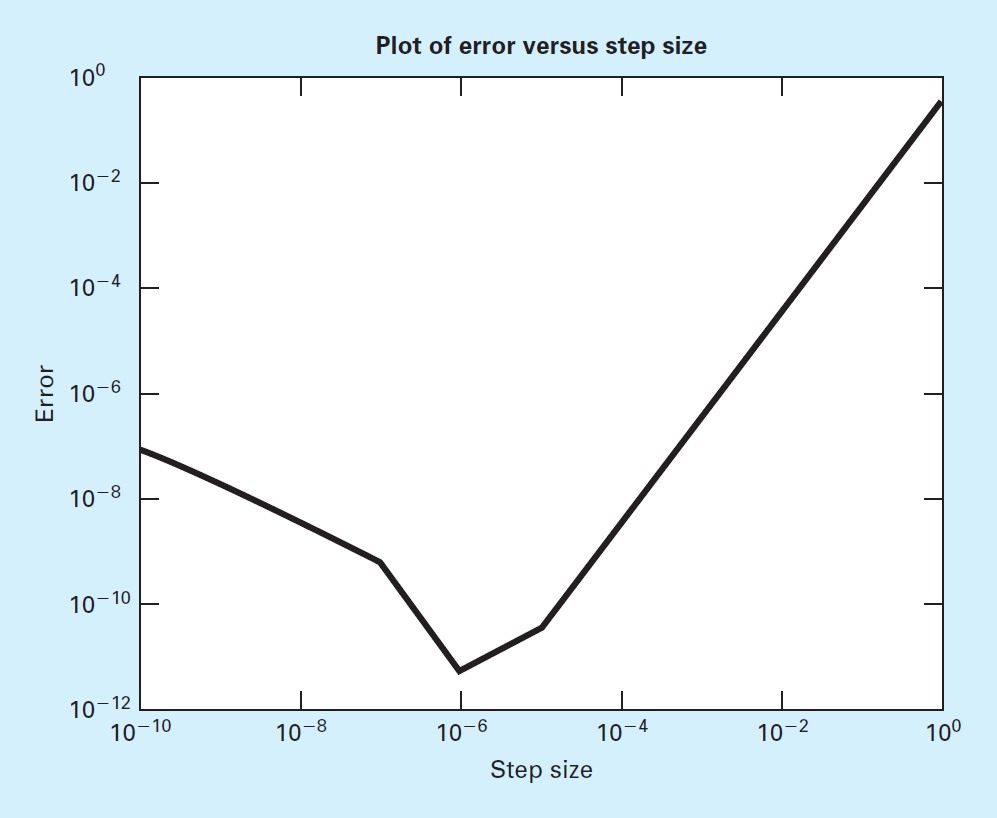
\includegraphics[width=0.75\linewidth]{./images/fig_4_12}
    \end{figure}
\end{example}


\subsection{Control of Numerical Errors}
\noindent
For most practical cases, we do not know the exact error associated with numerical methods.
The exception, of course, is when we know the exact solution, which makes our numerical
approximations unnecessary. Therefore, for most engineering and scientific applications we
must settle for some estimate of the error in our calculations.

There are no systematic and general approaches to evaluating numerical errors for all
problems. In many cases error estimates are based on the experience and judgment of the
engineer or scientist.

Although error analysis is to a certain extent an art, there are several practical programming
guidelines we can suggest. First and foremost, avoid subtracting two nearly
equal numbers. Loss of significance almost always occurs when this is done. Sometimes
you can rearrange or reformulate the problem to avoid subtractive cancellation. If this is not
possible, you may want to use extended-precision arithmetic. Furthermore, when adding
and subtracting numbers, it is best to sort the numbers and work with the smallest numbers
first. This avoids loss of significance.

Beyond these computational hints, one can attempt to predict total numerical errors
using theoretical formulations. The Taylor series is our primary tool for analysis of such
errors. Prediction of total numerical error is very complicated for even moderately sized problems
and tends to be pessimistic. Therefore, it is usually attempted for only small-scale tasks.

The tendency is to push forward with the numerical computations and try to estimate
the accuracy of your results. This can sometimes be done by seeing if the results satisfy
some condition or equation as a check. Or it may be possible to substitute the results back
into the original equation to check that it is actually satisfied.

Finally you should be prepared to perform numerical experiments to increase your
awareness of computational errors and possible ill-conditioned problems. Such experiments
may involve repeating the computations with a different step size or method and
comparing the results. We may employ sensitivity analysis to see how our solution changes
when we change model parameters or input values. We may want to try different numerical
algorithms that have different theoretical foundations, are based on different computational
strategies, or have different convergence properties and stability characteristics.

When the results of numerical computations are extremely critical and may involve
loss of human life or have severe economic ramifications, it is appropriate to take special
precautions. This may involve the use of two or more independent groups to solve the same
problem so that their results can be compared.

The roles of errors will be a topic of concern and analysis in all sections of this book.
We will leave these investigations to specific sections.\\
\bigskip


\section[BLUNDERS, MODEL ERRORS, AND DATA UNCERTAINTY]{BLUNDERS, MODEL ERRORS, AND DATA UNCERTAINTY}
\noindent
Although the following sources of error are not directly connected with most of the numerical
methods in this book, they can sometimes have great impact on the success of a
modeling effort. Thus, they must always be kept in mind when applying numerical techniques
in the context of real-world problems.\\

\subsection{Blunders}
\noindent
We are all familiar with gross errors, or blunders. In the early years of computers, erroneous
numerical results could sometimes be attributed to malfunctions of the computer itself.
Today, this source of error is highly unlikely, and most blunders must be attributed to human
imperfection.

Blunders can occur at any stage of the mathematical modeling process and can contribute
to all the other components of error. They can be avoided only by sound knowledge
of fundamental principles and by the care with which you approach and design your solution
to a problem.

Blunders are usually disregarded in discussions of numerical methods. This is no doubt
due to the fact that, try as we may, mistakes are to a certain extent unavoidable. However, we
believe that there are a number of ways in which their occurrence can be minimized. In particular,
the good programming habits that were outlined in Chap. 3 are extremely useful for
mitigating programming blunders. In addition, there are usually simple ways to check
whether a particular numerical method is working properly. Throughout this book, we discuss
ways to check the results of numerical calculations.\\

\subsection{Model Errors}
\noindent
\emph{Model errors} relate to bias that can be ascribed to incomplete mathematical models. An example
of a negligible model error is the fact that Newton's second law does not account for
relativistic effects. This does not detract from the adequacy of the solution in Example 1.1
because these errors are minimal on the time and space scales associated with the bungee
jumper problem.
However, suppose that air resistance is not proportional to the square of the fall velocity,
as in Eq. (1.7), but is related to velocity and other factors in a different way. If such were the
case, both the analytical and numerical solutions obtained in Chap. 1 would be erroneous because
of model error.You should be cognizant of this type of error and realize that, if you are
working with a poorly conceived model, no numerical method will provide adequate results.\\

\subsection{Data Uncertainty}
\noindent
Errors sometimes enter into an analysis because of uncertainty in the physical data on which
a model is based. For instance, suppose we wanted to test the bungee jumper model by having
an individual make repeated jumps and then measuring his or her velocity after a specified
time interval. Uncertainty would undoubtedly be associated with these measurements, as
the parachutist would fall faster during some jumps than during others. These errors can exhibit
both inaccuracy and imprecision. If our instruments consistently underestimate or overestimate
the velocity, we are dealing with an inaccurate, or biased, device. On the other hand,
if the measurements are randomly high and low, we are dealing with a question of precision.

Measurement errors can be quantified by summarizing the data with one or more wellchosen
statistics that convey as much information as possible regarding specific characteristics
of the data. These descriptive statistics are most often selected to represent (1) the
location of the center of the distribution of the data and (2) the degree of spread of the data.
As such, they provide a measure of the bias and imprecision, respectively.We will return to
the topic of characterizing data uncertainty when we discuss regression in Part Four.

Although you must be cognizant of blunders, model errors, and uncertain data, the numerical
methods used for building models can be studied, for the most part, independently
of these errors. Therefore, for most of this book, we will assume that we have not made gross
errors, we have a sound model, and we are dealing with error-free measurements. Under
these conditions, we can study numerical errors without complicating factors.\\
\bigskip

\noindent\textbf{PROBLEMS}\\

\begin{multicols}{2}
    \noindent\textbf{4.1} The ``divide and average'' method, an old-time method
    for approximating the square root of any positive number a,
    can be formulated as\\

    $x = \dfrac{x+a/x}{2}$\\

    \noindent
    Write a well-structured function to implement this algorithm
    based on the algorithm outlined in Fig. 4.2.\\

    \noindent\textbf{4.2} Convert the following base-2 numbers to base 10:
    \textbf{(a)} 1011001, \textbf{(b)} 0.01011, and \textbf{(c)} 110.01001.\\

    \noindent\textbf{4.3} Convert the following base-8 numbers to base 10:
    61,565 and 2.71.\\

    \noindent\textbf{4.4} For computers, the machine epsilon $\epsilon$ can also be
    thought of as the smallest number that when added to one
    gives a number greater than 1. An algorithm based on this
    idea can be developed as\\
    Step 1: Set $\epsilon = 1$\\
    Step 2: If $1 + \epsilon$ is less than or equal to 1, then go to Step 5.
    Otherwise go to Step 3.\\
    Step 3: $\epsilon = \epsilon/2$\\
    Step 4: Return to Step 2\\
    Step 5: $\epsilon = 2 \times \epsilon$\\

    \noindent Write your own M-file based on this algorithm to determine
    the machine epsilon. Validate the result by comparing it with
    the value computed with the built-in function \texttt{eps}.\\

    \noindent\textbf{4.5} In a fashion similar to Prob. 4.4, develop your own
    M-file to determine the smallest positive real number used in
    MATLAB. Base your algorithm on the notion that your computer
    will be unable to reliably distinguish between zero and
    a quantity that is smaller than this number. Note that the
    result you obtain will differ from the value computed with
    \texttt{realmin}.Challenge question: Investigate the results by
    taking the base-2 logarithm of the number generated by your
    code and those obtained with \texttt{realmin}.\\

    \noindent\textbf{4.6} Although it is not commonly used, MATLAB allows
    numbers to be expressed in single precision. Each value
    is stored in 4 bytes with 1 bit for the sign, 23 bits for the
    mantissa, and 8 bits for the signed exponent. Determine the
    smallest and largest positive floating-point numbers as well
    as the machine epsilon for single precision representation.
    Note that the exponents range from -126 to 127.\\

    \noindent\textbf{4.7} For the hypothetical base-10 computer in Example 4.2,
    prove that the machine epsilon is 0.05.\\

    \noindent\textbf{4.8} The derivative of $f(x) = 1/(1-3x^2)$ is given by\\

    $\dfrac{6x}{(1-3x^2)^2}$\\

    \noindent Do you expect to have difficulties evaluating this function
    at x = 0.577? Try it using 3- and 4-digit arithmetic with
    chopping.\\

    \noindent\textbf{4.9} \textbf{(a)} Evaluate the polynomial\\

    $y = x^3 - 7x^2 +8x - 0.35$\\

    \noindent at x = 1.37. Use 3-digit arithmetic with chopping. Evaluate
    the percent relative error.\\
    
    \noindent\textbf{(b)} Repeat \textbf{(a)} but express $y$ as\\

    $y = ((x-7)x+8)x-0.35$\\

    \noindent Evaluate the error and compare with part \textbf{(a)}.\\

    \noindent\textbf{4.10} The following infinite series can be used to approximate
    $e^x$:\\
    
    $e^x = 1+x+\dfrac{x^2}{2}+\dfrac{x^3}{3!}+\hdots +\dfrac{x^n}{n!}$\\

    \noindent\textbf{(a)} Prove that this Maclaurin series expansion is a special
    case of the Taylor series expansion (Eq. 4.13) with $x_i=0$ and $h = x$.\\

    \noindent\textbf{(b)} Use the Taylor series to estimate $f(x) = e^{-x}$ at $x_{i+1}= 1$
    for $x_i = 0.25$. Employ the zero-, first-, second-, 
    and third-order versions and compute the $\left\lvert \epsilon_t \right\rvert$  for each case.\\

    \noindent\textbf{4.11} The Maclaurin series expansion for $cos x$ is\\

    $cosx = 1-\dfrac{x^2}{2}+\dfrac{x^4}{4!}-\dfrac{x^6}{6!}+\dfrac{x^8}{8!}-\hdots$\\

    \noindent Starting with the simplest version, $cos x = 1$, add terms one
    at a time to estimate $cos(\pi/4)$. After each new term is added,
    compute the true and approximate percent relative errors.
    Use your pocket calculator or MATLAB to determine the
    true value. Add terms until the absolute value of the approximate
    error estimate falls below an error criterion conforming
    to two significant figures.\\

    \noindent\textbf{4.12} Perform the same computation as in Prob. 4.11, but
    use the Maclaurin series expansion for the $sin x$ to estimate
    $sin(\pi/4)$.\\

    $sinx = x-\dfrac{x^3}{3!}+\dfrac{x^5}{5!}-\dfrac{x^7}{7!}+\hdots$\\

    \noindent\textbf{4.13} Use zero- through third-order Taylor series expansions
    to predict $f (3)$ for\\

    $f(x) = 25x^3-6x^2+7x-88$\\

    \noindent using a base point at $x = 1$. Compute the true percent relative
    error $\epsilon_t$ for each approximation.\\

    \noindent\textbf{4.14} Prove that Eq. (4.11) is exact for all values of $x$ 
    if $f(x) = ax^2+bx+c$\\

    \noindent\textbf{4.15} Use zero- through fourth-order Taylor series expansions
    to predict $f(2)$ for $f (x) =$ ln $x$ using a base point at $ x = 1$.
    Compute the true percent relative error $\epsilon_t$ for each approximation.
    Discuss the meaning of the results.\\

    \noindent\textbf{4.16} Use forward and backward difference approximations
    of $O(h)$ and a centered difference approximation of $O(h^2)$ to
    estimate the first derivative of the function examined in
    Prob. 4.13. Evaluate the derivative at $x = 2$ using a step size
    of $h = 0.25$. Compare your results with the true value of the
    derivative. Interpret your results on the basis of the remainder
    term of the Taylor series expansion.\\

    \noindent\textbf{4.17} Use a centered difference approximation of $O(h^2)$ to
    estimate the second derivative of the function examined in
    Prob. 4.13. Perform the evaluation at $x = 2$ using step sizes
    of $h = 0.2$ and $0.1$. Compare your estimates with the true
    value of the second derivative. Interpret your results on the
    basis of the remainder term of the Taylor series expansion.\\

    \noindent\textbf{4.18} If $\left\lvert x \right\rvert < 1$ it is known that\\

    $\dfrac{1}{1-x} = 1+x+x^2+x^3+\hdots$\\

    \noindent Repeat Prob. 4.11 for this series for $x = 0.1$.\\

    \noindent\textbf{4.19} To calculate a planet's space coordinates, we have to
    solve the function\\

    $f(x)=x-1-0.5sinx$\\

    \noindent Let the base point be $a = x_i = \pi/2$ on the interval $[0, \pi]$.
    Determine the highest-order Taylor series expansion resulting
    in a maximum error of 0.015 on the specified interval.
    The error is equal to the absolute value of the difference
    between the given function and the specific Taylor series
    expansion. (Hint: Solve graphically.)\\

    \noindent\textbf{4.20} Consider the function $f(x) = x^3 - 2x + 4$ on the interval
    [-2, 2] with $h = 0.25$. Use the forward, backward, and
    centered finite difference approximations for the first and
    second derivatives so as to graphically illustrate which approximation
    is most accurate. Graph all three first-derivative
    finite difference approximations along with the theoretical,
    and do the same for the second derivative as well.\\

    \noindent\textbf{4.21} Derive Eq. (4.30).\\

    \noindent\textbf{4.22} Repeat Example 4.5, but for $f (x) = cos(x)$ at $x = \pi/6$.\\

    \noindent\textbf{4.23} Repeat Example 4.5, but for the forward divided difference (Eq. 4.21).\\

    \noindent\textbf{4.24} One common instance where subtractive cancellation
    occurs involves finding the roots of a parabola, $ax^2+bx+c$, with the quadratic formula:\\

    $x = \dfrac{-b \pm \sqrt{b^2-4ac}}{2a}$\\

    \noindent For cases where $b^2 >> 4ac$, the difference in the numerator
    can be very small and roundoff errors can occur. In such
    cases, an alternative formulation can be used to minimize
    subtractive cancellation:\\

    $x = \dfrac{-2c}{b\pm \sqrt{b^2-4ac}}$\\

    \noindent Use 5-digit arithmetic with chopping to determine the roots
    of the following equation with both versions of the quadratic
    formula.\\

    $x^2 - 5000.002x+10$\\
\end{multicols}
\end{document}
